% Options for packages loaded elsewhere
\PassOptionsToPackage{unicode}{hyperref}
\PassOptionsToPackage{hyphens}{url}
%
\documentclass[
]{article}
\usepackage{lmodern}
\usepackage{amssymb,amsmath}
\usepackage{ifxetex,ifluatex}
\ifnum 0\ifxetex 1\fi\ifluatex 1\fi=0 % if pdftex
  \usepackage[T1]{fontenc}
  \usepackage[utf8]{inputenc}
  \usepackage{textcomp} % provide euro and other symbols
\else % if luatex or xetex
  \usepackage{unicode-math}
  \defaultfontfeatures{Scale=MatchLowercase}
  \defaultfontfeatures[\rmfamily]{Ligatures=TeX,Scale=1}
\fi
% Use upquote if available, for straight quotes in verbatim environments
\IfFileExists{upquote.sty}{\usepackage{upquote}}{}
\IfFileExists{microtype.sty}{% use microtype if available
  \usepackage[]{microtype}
  \UseMicrotypeSet[protrusion]{basicmath} % disable protrusion for tt fonts
}{}
\makeatletter
\@ifundefined{KOMAClassName}{% if non-KOMA class
  \IfFileExists{parskip.sty}{%
    \usepackage{parskip}
  }{% else
    \setlength{\parindent}{0pt}
    \setlength{\parskip}{6pt plus 2pt minus 1pt}}
}{% if KOMA class
  \KOMAoptions{parskip=half}}
\makeatother
\usepackage{xcolor}
\IfFileExists{xurl.sty}{\usepackage{xurl}}{} % add URL line breaks if available
\IfFileExists{bookmark.sty}{\usepackage{bookmark}}{\usepackage{hyperref}}
\hypersetup{
  pdftitle={Especificación de diseño},
  hidelinks,
  pdfcreator={LaTeX via pandoc}}
\urlstyle{same} % disable monospaced font for URLs
\usepackage{graphicx}
\makeatletter
\def\maxwidth{\ifdim\Gin@nat@width>\linewidth\linewidth\else\Gin@nat@width\fi}
\def\maxheight{\ifdim\Gin@nat@height>\textheight\textheight\else\Gin@nat@height\fi}
\makeatother
% Scale images if necessary, so that they will not overflow the page
% margins by default, and it is still possible to overwrite the defaults
% using explicit options in \includegraphics[width, height, ...]{}
\setkeys{Gin}{width=\maxwidth,height=\maxheight,keepaspectratio}
% Set default figure placement to htbp
\makeatletter
\def\fps@figure{htbp}
\makeatother
\setlength{\emergencystretch}{3em} % prevent overfull lines
\providecommand{\tightlist}{%
  \setlength{\itemsep}{0pt}\setlength{\parskip}{0pt}}
\setcounter{secnumdepth}{-\maxdimen} % remove section numbering

\title{Especificación de diseño}
\author{}
\date{}

\begin{document}
\maketitle

\hypertarget{introducciuxf3n}{%
\section{Introducción}\label{introducciuxf3n}}

Este anexo recoge todos los aspectos relacionados con el diseño de la
aplicación, incluyendo aquellos que forman parte de los complementos
desarrollados. Con ello se pretende conocer en detalle tanto su
funcionamiento como su estructura.

\hypertarget{diseuxf1o-de-datos}{%
\section{Diseño de datos}\label{diseuxf1o-de-datos}}

Para la gestión de datos, la aplicación hace uso de las siguientes
entidades:

\begin{itemize}
\tightlist
\item
  \textbf{Ítem} (\emph{Item}): es la materia prima de la aplicación.
  Agrupa toda la información de cada uno de los datos existentes en la
  plataforma. La mayor parte de entidades están relacionadas con esta
  entidad.
\item
  \textbf{Conjunto de elementos} (\emph{ElementSet}): representa un
  esquema de metadatos.
\item
  \textbf{Elemento} (\emph{Element}): representa un elemento (metadato)
  de un esquema de metadatos. Está relacionado con un conjunto de
  elementos (\emph{ElementSet}).
\item
  \textbf{Texto del elemento} (\emph{ElementText}): representa el
  contenido de un elemento para una determinada entidad (e.g. ítem).
\item
  \textbf{Colección} (\emph{Collection}): representa una agrupación de
  ítems.
\item
  \textbf{Etiqueta} (\emph{Tag}): representa una etiqueta con texto
  simple.
\item
  \textbf{Registros etiqueta} (\emph{RecordsTag}): relaciona una
  etiqueta con uno o varios ítems.
\item
  \textbf{Tipo de ítem} (\emph{ItemType}): permite asignar un tipo a un
  ítem y añadirle a este elementos (metadatos) específicos del tipo.
\item
  \textbf{Elementos de tipos de ítem}: (\emph{ItemTypesElements}):
  representa la relación entre un elemento (metadato) y un tipo de ítem.
\item
  \textbf{Fichero} (\emph{File}): representa un fichero asignado a un
  ítem.
\item
  \textbf{Fichero de colección} (\emph{CollectionFile}): representa un
  fichero asignado a una colección.
\item
  \textbf{Localización} (\emph{Location}): representa la localización de
  un ítem.
\item
  \textbf{Localización rectangular} (\emph{BoxLocation}): representa la
  localización rectangular de un ítem.
\end{itemize}

\begin{figure}
\hypertarget{e-r-uml}{%
\centering
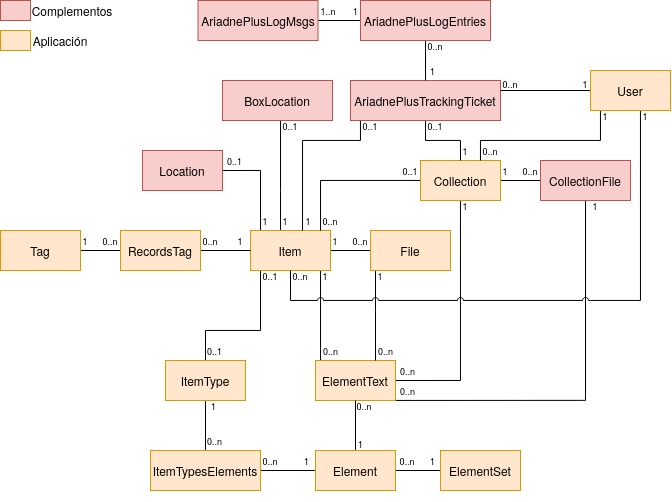
\includegraphics{../_static/images/e-r-uml.png}
\caption{Diagrama E/R de datos relacionados con la gestión de
datos.}\label{e-r-uml}
}
\end{figure}

\hypertarget{diseuxf1o-arquitectuxf3nico}{%
\section{Diseño arquitectónico}\label{diseuxf1o-arquitectuxf3nico}}

Como es lógico, el diseño de los complementos (\emph{plugins})
desarrollados se ha visto condicionado por el diseño de la aplicación
para la que iban dirigidos.

\hypertarget{modelo-vista-controlador-mvc}{%
\subsection{Modelo-Vista-Controlador
(MVC)}\label{modelo-vista-controlador-mvc}}

La aplicación propuesta usa el patrón de diseño
\emph{modelo-vista-controlador} (\emph{MVC}), el cual ofrece una serie
de consejos para organizar correctamente el código desarrollado y
facilitar así su mantenimiento.

Las aplicaciones que siguen este patrón contienen clases que implementan
la lógica de negocio (\emph{modelos}), ficheros con código HTML y PHP
(\emph{vistas}), y clases que interactúan con los usuarios
(\emph{controladores}). En las vistas no se ha utilizado el término
\emph{clase} para referirnos a estas ya que, por lo general, son
documentos simples que contienen fragmentos de código HTML y PHP.

Por tanto, podemos deducir que el diseño se divide en tres capas:

\begin{itemize}
\tightlist
\item
  \emph{Modelo}: modifica, gestiona y actualiza los datos de la
  aplicación. En nuestro caso, al contar con una única base de datos, es
  la capa donde se encuentra el código relacionado con las consultas,
  búsquedas, filtros y actualizaciones.
\item
  \emph{Vista}: muestra al usuario final la interfaz gráfica de la
  aplicación, es decir, las páginas, ventanas, formularios, etc. En
  términos de programación se correspondería con el \emph{frontend}. En
  la aplicación se correspondería con la interfaz pública y de
  administración.
\item
  \emph{Controlador}: gestiona, atiende y procesa las peticiones
  realizadas por parte de los usuarios. A través de esta capa se
  comunican el \emph{modelo} y la \emph{vista}. El \emph{controlador}
  solicita los datos necesarios al \emph{modelo}, se manipulan acorde a
  la petición del usuario, y se entregan a la \emph{vista} de forma que
  el usuario pueda visualizar los resultados esperados.
\end{itemize}

\begin{figure}
\hypertarget{da-mvc}{%
\centering
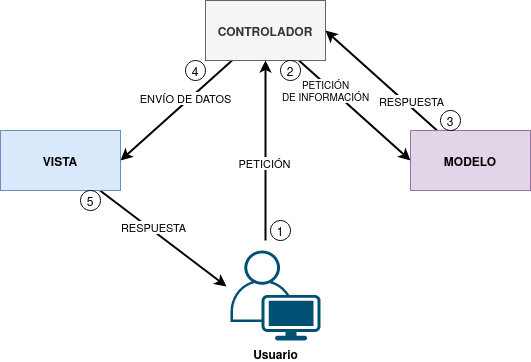
\includegraphics{../_static/images/mvc.png}
\caption{Diagrama que muestra la relación entre el Modelo, Vista y
Controlador del patrón MVC.}\label{da-mvc}
}
\end{figure}

En el siguiente diagrama se muestra el comportamiento de la aplicación
ante una \emph{petición HTTP}.

\begin{figure}
\hypertarget{mvc-full}{%
\centering
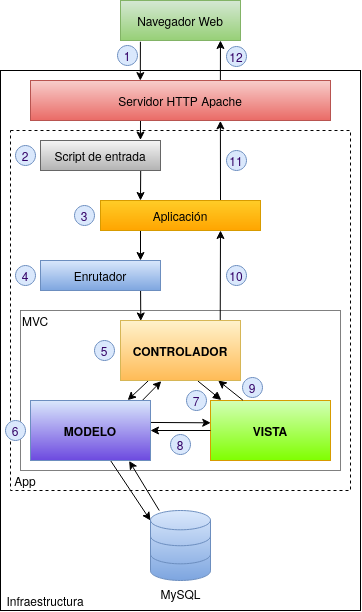
\includegraphics{../_static/images/mvc-full.png}
\caption{Diagrama que muestra el comportamiento de la aplicación ante
una petición HTTP.}\label{mvc-full}
}
\end{figure}

\begin{enumerate}
\def\labelenumi{\arabic{enumi}.}
\tightlist
\item
  El usuario entra a la aplicación a través de su navegador web con la
  dirección de la aplicación (e.g. \emph{http://miaplicación.es}).
\item
  El servidor web con ayuda de la extensión PHP ejecuta el script de
  entrada (\emph{index.php}).
\item
  Se crea una instancia de la aplicación (\emph{Application}).
\item
  La aplicación usa el componente enrutador (\emph{router}) para
  analizar la URL con la que se ha accedido y determinar qué controlador
  procesará la petición. Si la ruta existe, se instancia al
  \emph{controlador} y se llama a la acción involucrada.
\item
  El método de la \emph{acción} recupera los parámetros de las variables
  globales (e.g. \emph{GET}, \emph{POST}, \emph{FILES}, etc.) y los
  procesa haciendo uso de los métodos de las clases \emph{modelo}.
\item
  Las clases \emph{modelo} recogen los datos provistos por el
  controlador y llevan a cabo las tareas oportunas (e.g recuperar,
  añadir, eliminar o modificar datos de la base de datos).
\item
  Después de llamar a los \emph{modelos}, se pasa a la \emph{vista}
  correspondiente para renderizar la página HTML.
\item
  La \emph{vista} podría, en caso de necesitarlo, consultar datos del
  \emph{modelo} para la renderización.
\item
  La \emph{vista} produce la salida HTML.
\item
  El \emph{controlador} envía los datos a la instancia de la
  \emph{aplicación}.
\item
  Se envía la respuesta HTTP al \emph{servidor web}.
\item
  La respuesta HTTP es enviada al navegador del \emph{cliente}
  (usuario).
\end{enumerate}

\hypertarget{diseuxf1o-de-paquetes}{%
\subsection{Diseño de paquetes}\label{diseuxf1o-de-paquetes}}

Antes de mostrar cómo se encuentran organizados los complementos
(\emph{plugins}) que se han desarrollado, se va a realizar un estudio de
cómo lo están los paquetes principales de la aplicación.

\begin{figure}
\hypertarget{da-pck-1}{%
\centering
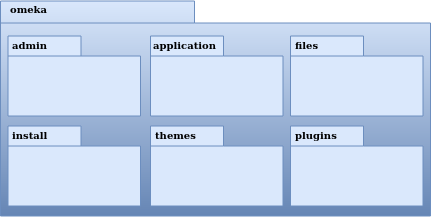
\includegraphics{../_static/images/pck-1.png}
\caption{Diagrama de paquetes de la aplicación.}\label{da-pck-1}
}
\end{figure}

\begin{itemize}
\tightlist
\item
  \emph{omeka.admin} : contiene todas las clases de cada una de las
  \emph{vistas} del área de administración.
\item
  \emph{omeka.application}: contiene la aplicación. Alberga todo el
  sistema \emph{MVC}, así como las configuraciones y servicios
  utilizados.
\item
  \emph{omeka.files}: recoge todos los ficheros almacenados en la
  plataforma.
\item
  \emph{omeka.install}: contiene los ficheros de instalación inicial,
  necesarios para inicializar los parámetros principales de la
  aplicación.
\item
  \emph{omeka.themes}: recoge las plantillas de diseño (\emph{themes})
  utilizadas para personalizar el área pública (\emph{frontend}) de la
  aplicación.
\item
  \emph{omeka.plugins}: contiene todos los complementos (\emph{plugins})
  utilizados para añadir nuevas funcionalidades a la aplicación.
\end{itemize}

De todos estos paquetes únicamente se especificará en detalle el paquete
\emph{plugins} por el hecho de que sólo se ha trabajado en la creación,
modificación e instalación de complementos (\emph{plugins}).

\hypertarget{complementos-plugins}{%
\subsubsection{\texorpdfstring{Complementos
(\emph{plugins})}{Complementos (plugins)}}\label{complementos-plugins}}

Para obtener una visión más clara de cómo están organizados los
complementos (\emph{plugins}) se mostrará su estructura de directorios
general.

\begin{figure}
\hypertarget{da-pck-2}{%
\centering
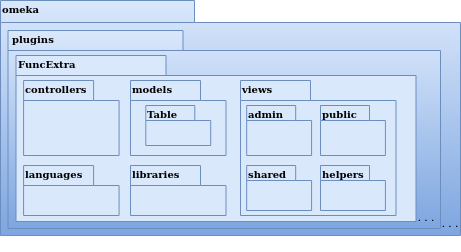
\includegraphics{../_static/images/pck-2.png}
\caption{Diagrama de paquetes del complemento ficticio
\emph{FuncExtra}.}\label{da-pck-2}
}
\end{figure}

\begin{itemize}
\item
  \emph{omeka.plugins.FuncExtra}: representa el nivel superior del
  complemento. Alberga todo el sistema \emph{MVC} del complemento.
\item
  \emph{omeka.plugins.FuncExtra.controllers}: contiene todas las clases
  de la capa \emph{controlador}.
\item
  \emph{omeka.plugins.FuncExtra.libraries}: contiene clases externas
  utilizadas por el complemento.
\item
  \emph{omeka.plugins.FuncExtra.languages}: contiene las traducciones
  del texto existente en el complemento.
\item
  \emph{omeka.plugins.FuncExtra.models}: contiene las clases de la capa
  \emph{modelo}. Permite al complemento crear y gestionar sus propias
  tablas en la base de datos.

  \begin{quote}
  \begin{itemize}
  \tightlist
  \item
    \emph{omeka.plugins.FuncExtra.Table}: contiene parte de las clases
    de la capa \emph{modelo}.
  \end{itemize}
  \end{quote}
\item
  \emph{omeka.plugins.FuncExtra.views}: contiene los archivos (que no
  clases) de la capa \emph{vista}.

  \begin{quote}
  \begin{itemize}
  \tightlist
  \item
    \emph{omeka.plugins.FuncExtra.views.admin}: contiene las
    \emph{vistas} solo visibles en el área de administración.
  \item
    \emph{omeka.plugins.FuncExtra.views.public}: contiene las
    \emph{vistas} solo visibles en el área pública.
  \item
    \emph{omeka.plugins.FuncExtra.views.shared}: contiene las
    \emph{vistas} visibles en ambas áreas.
  \end{itemize}
  \end{quote}
\end{itemize}

A continuación, se muestran los paquetes de todos los complementos
instalados en la aplicación.

\begin{figure}
\hypertarget{da-pck-2-1}{%
\centering
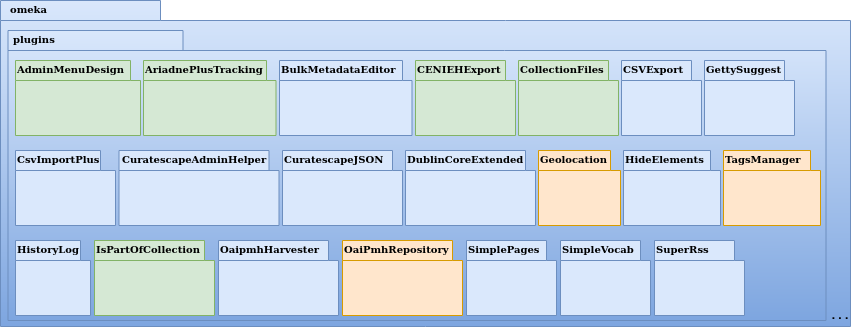
\includegraphics{../_static/images/pck-2-1.png}
\caption{Paquetes de los complementos instalados en la
aplicación.}\label{da-pck-2-1}
}
\end{figure}

Son un total de 21 complementos, de los cuales 6 han sido creados
específicamente para el proyecto (verdes) y el resto (azules) han sido
recogidos de la página oficial de Omeka o de repositorios externos. De
estos últimos se han modificado 3 para añadir nuevas funcionalidades
(naranjas).

\begin{itemize}
\tightlist
\item
  \emph{omeka.plugins.AdminMenuDesign}: permite ordenar las entradas del
  menú principal de navegación del área de administración en secciones
  (submenús).
\item
  \emph{omeka.plugins.AriadnePlusTracking}: implementa todas las
  funcionalidades relacionadas con los tickets de seguimiento para los
  procesos de integración en ARIADNEplus.
\item
  \emph{omeka.plugins.BulkMetadataEditor}: permite añadir, editar o
  eliminar metadatos de ítems de forma masiva.
\item
  \emph{omeka.plugins.CENIEHExport}: permite exportar ítems y
  colecciones en un formato compatible con ARIADNEplus.
\item
  \emph{omeka.plugins.CollectionFiles}: permite asociar ficheros a
  colecciones.
\item
  \emph{omeka.plugins.GettySuggest}: permite sugerir términos de los
  vocabularios Getty durante el relleno de un metadato.
\item
  \emph{omeka.plugins.CsvImportPlus}: permite importar elementos
  (metadatos, localizaciones, etc.) en formato CSV y gestionar las
  importaciones.
\item
  \emph{omeka.plugins.CuratescapeAdminHelper}: implementa
  funcionalidades que brindan ayuda a los administradores de la
  aplicación.
\item
  \emph{omeka.plugins.CuratescapeJSON}: implementa funcionalidades para
  la plantilla de diseño (\emph{theme}).
\item
  \emph{omeka.plugins.DublinCoreExtended}: implementa nuevos elementos
  en el esquema de metadatos (\emph{ElementSet}) \emph{Dublin Core}.
\item
  \emph{omeka.plugins.Geolocation}: implementa diversas funcionalidades
  relacionadas con la geolocalización de los ítems.
\item
  \emph{omeka.plugins.HideElements}: permite ocultar elementos de los
  esquemas de metadatos (\emph{ElementSet}) existentes en la plataforma.
\item
  \emph{omeka.plugins.TagsManager}: añade funcionalidades relacionadas
  con las etiquetas (\emph{tags}).
\item
  \emph{omeka.plugins.HistoryLog}: permite llevar un registro detallado
  de todas las acciones (eliminar, editar, crear, etc.) ejecutadas en la
  plataforma.
\item
  \emph{omeka.plugins.AutoDublinCore}: permite automatizar el relleno de
  algunos elementos del esquema \emph{Dublin Core}.
\item
  \emph{omeka.plugins.OaipmhHarvester}: permite recolectar metadatos de
  otros repositorios web y gestionar las recolecciones ejecutadas.
\item
  \emph{omeka.plugins.OaiPmhRepository}: permite que otros repositorios
  web recolecten metadatos de nuestra aplicación.
\item
  \emph{omeka.plugins.SimplePages}: permite añadir páginas simples como
  la de "About" al área pública.
\item
  \emph{omeka.plugins.SimpleVocab}: permite crear y gestionar
  vocabularios simples para elementos de un determinado esquema.
\item
  \emph{omeka.plugins.SuperRss}: muestra enlaces para compartir
  publicaciones (área pública) en redes sociales.
\end{itemize}

\hypertarget{diseuxf1o-de-clases}{%
\subsection{Diseño de clases}\label{diseuxf1o-de-clases}}

Cada complemento puede contar con las siguientes clases, de las cuales
sólo la primera es de uso obligatorio.

\begin{itemize}
\item
  \emph{FuncExtraPlugin}: representa la clase principal del complemento
  \emph{FuncExtra}. Permite definir las llamadas a "\emph{hooks}" y
  "\emph{filters}" y establecer las opciones de configuración del
  complemento.
\item
  \emph{FuncExtraRecord}: implementa la capa \emph{modelo} del
  complemento \emph{FuncExtra}. Cada complemento puede implementar
  varios \emph{modelos} o ninguno.

  \begin{quote}
  \begin{itemize}
  \tightlist
  \item
    \emph{Table\_FuncExtraRecord}: es parte de la implementación de la
    capa \emph{modelo}. Sobre él se implementan métodos para hacer
    búsquedas sobre la base de datos y obtener como resultado objetos de
    la clase \emph{FuncExtraRecord}.
  \end{itemize}
  \end{quote}
\item
  \emph{FuncExtra\_IndexController}: implementa la capa
  \emph{controlador} del complemento \emph{FuncExtra}. En este caso,
  implementaría el \emph{controlador} \emph{index}. Cada complemento
  puede implementar varios \emph{controladores} o ninguno.
\item
  \emph{FuncExtraHelper\_View\_Helper\_Extra}: implementa el ayudante
  \emph{Extra}. Este provee a las \emph{vistas} del complemento
  \emph{FuncExtra} métodos para llevar a cabo funciones complejas como,
  por ejemplo, añadir elementos a un formulario. Es una clase opcional.
\end{itemize}

\begin{figure}
\hypertarget{da-pck-3}{%
\centering
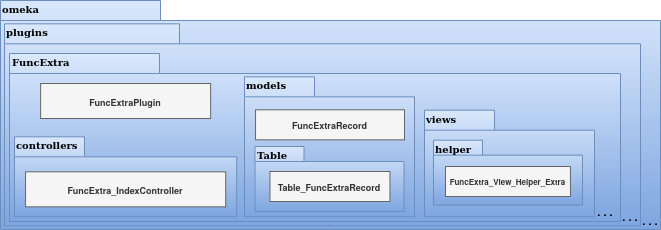
\includegraphics{../_static/images/pck-3.png}
\caption{Paquete tipo del complemento ficticio
FuncExtra.}\label{da-pck-3}
}
\end{figure}

Como se puede apreciar, el nombre de cada clase varía en función del
complemento al que pertenece y, en el caso de los \emph{modelos} y
\emph{controladores}, hay que considerar además el nombre del
\emph{modelo} o \emph{controlador} que se está implementando. Adoptando
estas medidas, se evitan posibles conflictos en la nomenclatura de las
clases.

En el siguiente diagrama se muestra la interacción entre los componentes
del complemento ficticio \emph{FuncExtra} y la aplicación principal.

\begin{figure}
\hypertarget{da-pck-4}{%
\centering
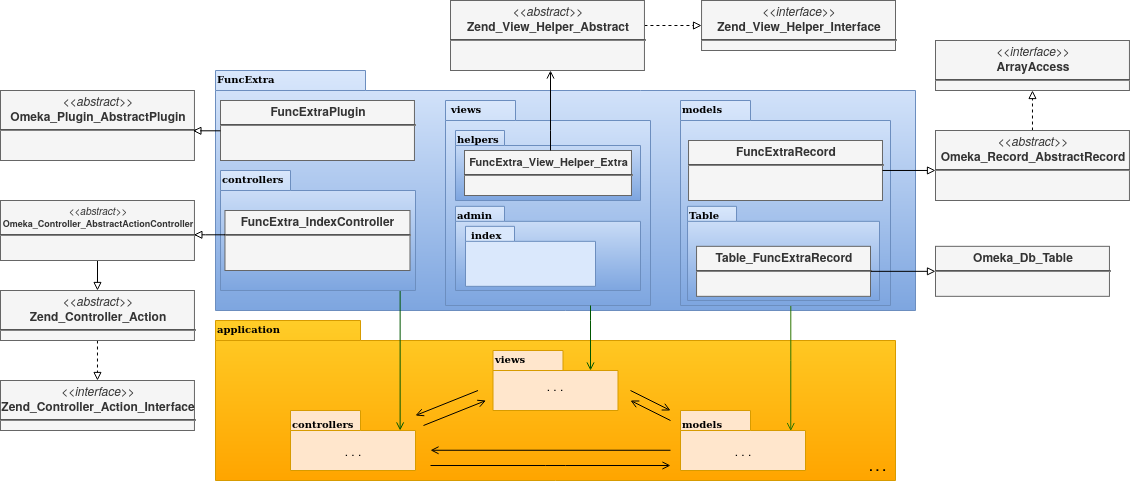
\includegraphics{../_static/images/pck-4.png}
\caption{Diagrama de clases del complemento ficticio
FuncExtra.}\label{da-pck-4}
}
\end{figure}

Vemos como las implementaciones de las tres capas del complemeto
\emph{FuncExtra} (\emph{models}, \emph{views} y \emph{controllers}) se
acoplan a las capas de la aplicación principal para despúes interactuar
entre ellas junto a todas las demás implementaciones de la aplicación,
incluyendo las de los otros complementos instalados. Este acoplamiento
hace posible que desde nuestro complemento se puedan reutilizar
implementaciones tanto de la propia aplicación como de los otros
complementos.

Además de estas clases, se pueden añadir clases externas dentro del
paquete \emph{libraries}.

El paquete \emph{views} no tiene clases por el hecho de que las
\emph{vistas} no son consideradas como clases en el patrón \emph{MVC},
sino una mezcla de código HTML y PHP.

Todos los complementos que se han instalado en la plataforma siguen esta
estructura, sin embargo, al ser todos los componentes opcionales (salvo
la clase principal), existen ciertas diferencias entre ellos.

A continuación, por motivos de brevedad, se mostrarán únicamente los
diagramas de clase de los seis complementos que se han desarrollado de
forma exclusiva para el proyecto. Aquellos que contengan paquetes nuevos
se explicará su significado.

\begin{figure}
\hypertarget{da-pck-5}{%
\centering
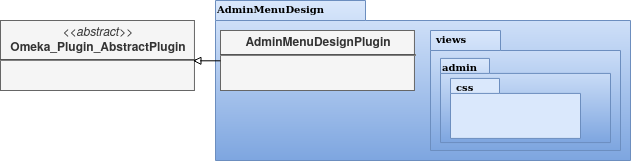
\includegraphics{../_static/images/pck-5.png}
\caption{Diagrama de clases del complemento
AdminMenuDesign.}\label{da-pck-5}
}
\end{figure}

En el complemento \emph{AdminMenuDesign} se hace uso de un paquete
nuevo:

\begin{itemize}
\tightlist
\item
  \emph{omeka.plugins.AriadnePlusTracking.views.css}: almacena las hojas
  de estilo \emph{CSS} utilizadas por las \emph{vistas} del complemento.
\end{itemize}

\begin{figure}
\hypertarget{da-pck-6}{%
\centering
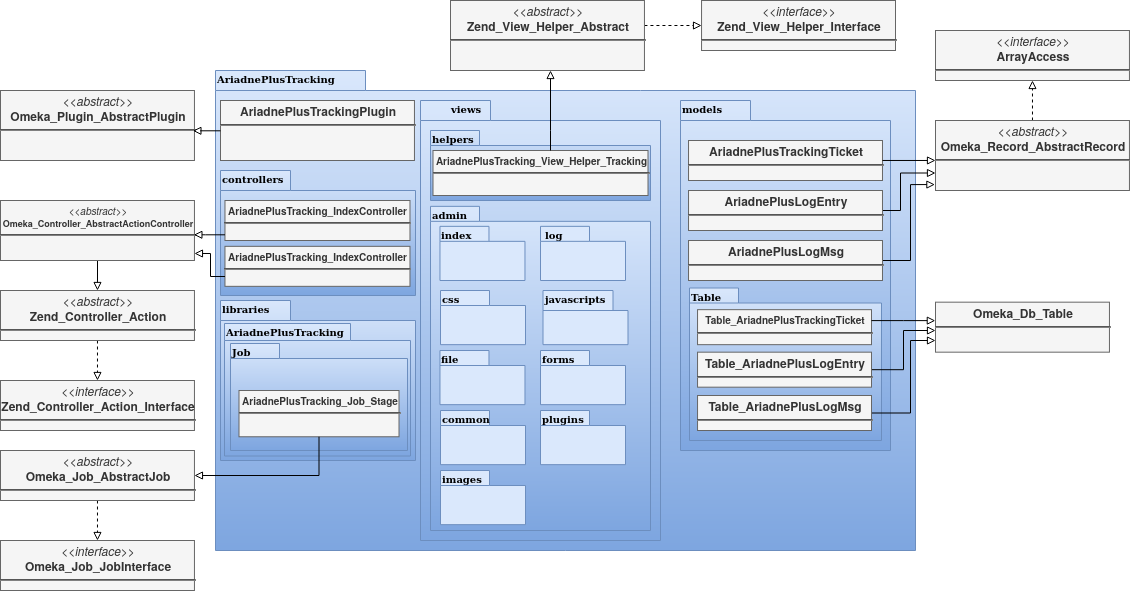
\includegraphics{../_static/images/pck-6.png}
\caption{Diagrama de clases del complemento
AriadnePlusTracking.}\label{da-pck-6}
}
\end{figure}

En el complemento \emph{AriadnePlusTracking} se utilizan varios paquetes
nuevos:

\begin{itemize}
\tightlist
\item
  \emph{omeka.plugins.AriadnePlusTracking.libraries.AriadnePlusTracking}:
  librería que implementa una nueva funcionalidad que permite ejecutar
  en segundo plano el proceso de cambio de fase del ticket.
\item
  \emph{omeka.plugins.AriadnePlusTracking.views.javascripts}: facilita
  el uso de \emph{JavaScrip} dentro de las vistas del complemento.
\item
  \emph{omeka.plugins.AriadnePlusTracking.views.file}: implementa la
  carga de ficheros. En este caso se utiliza para el campo "JSON file of
  your matchings to Getty AAT" del esquema Monitor.
\item
  \emph{omeka.plugins.AriadnePlusTracking.views.forms}: implementa los
  formularios de las \emph{vistas}.
\item
  \emph{omeka.plugins.AriadnePlusTracking.views.common}: implementa
  funcionalidades que se usan en varias \emph{vistas}.
\item
  \emph{omeka.plugins.AriadnePlusTracking.views.plugins}: implementa la
  página de configuración del complemento.
\item
  \emph{omeka.plugins.AriadnePlusTracking.views.images}: facilita el uso
  de imágenes dentro de las \emph{vistas} del complemento.
\end{itemize}

\begin{figure}
\hypertarget{da-pck-7}{%
\centering
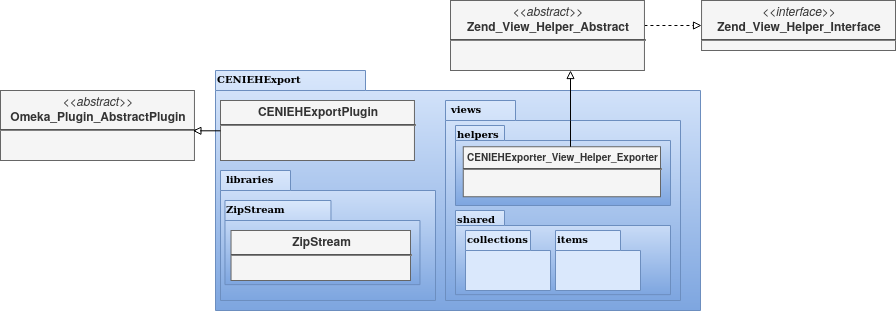
\includegraphics{../_static/images/pck-7.png}
\caption{Diagrama de clases del complemento
CENIEHExport.}\label{da-pck-7}
}
\end{figure}

En el complemento \emph{CENIEHExport} se hace uso de una nueva librería:

\begin{itemize}
\tightlist
\item
  \emph{ZipStream}: librería que permite comprimir varios ficheros
  (.xml) en formato \emph{.zip} de forma dinámica, sin tener que
  almacenar ningún fichero en el servidor.
\end{itemize}

\begin{figure}
\hypertarget{da-pck-8}{%
\centering
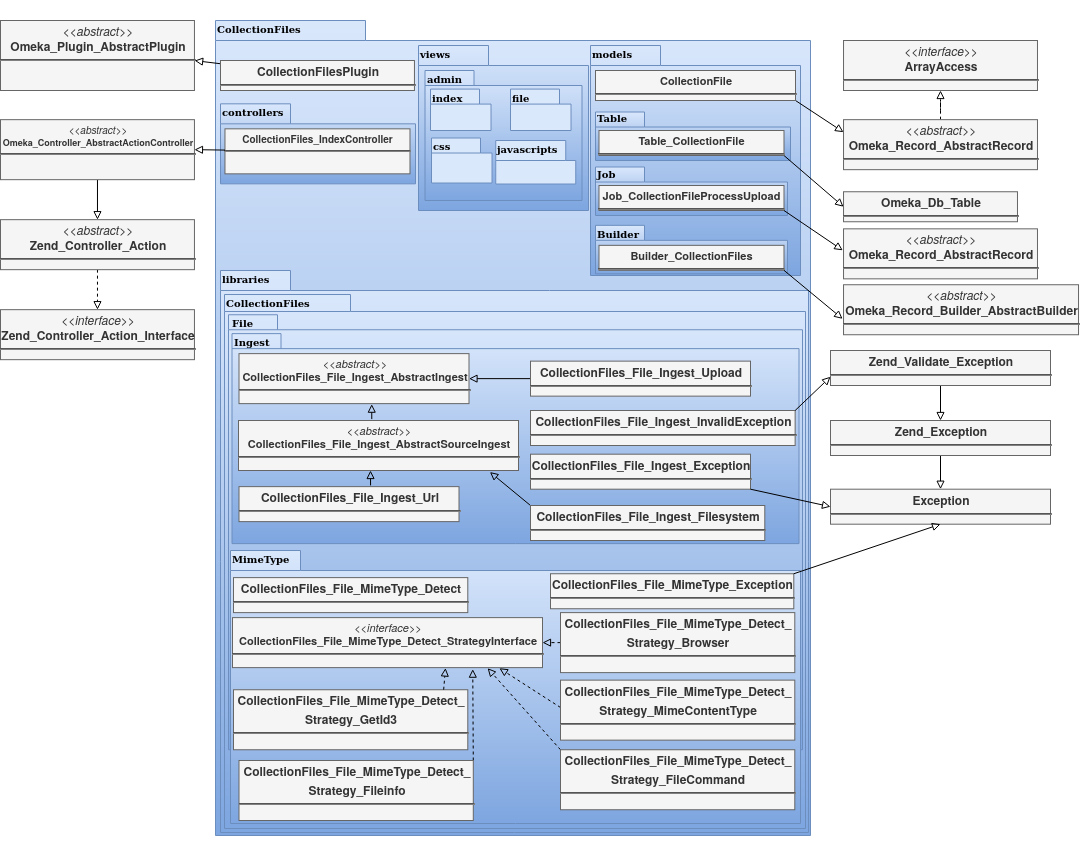
\includegraphics{../_static/images/pck-8.png}
\caption{Diagrama de clases del complemento
CollectionFiles}\label{da-pck-8}
}
\end{figure}

En el complemento \emph{CollectionFiles} se utiliza una nueva librería:

\begin{itemize}
\tightlist
\item
  \emph{CollectionFiles}: librería que implementa todas las
  funcionalidades que permiten asociar ficheros a colecciones.
\end{itemize}

Además, se utilizan dos paquetes nuevos:

\begin{itemize}
\tightlist
\item
  \emph{omeka.plugins.CollectionFiles.models.Builder}: paquete utilizado
  para implementar \emph{builders}. En este caso, implementa el
  \emph{builder} para el objeto \emph{CollectionFile}.
\item
  \emph{omeka.plugins.CollectionFiles.models.Job}: paquete utilizado
  para implementar \emph{jobs}. En este caso, el \emph{job} implementado
  procesa la carga de ficheros.
\end{itemize}

\begin{figure}
\hypertarget{da-pck-9}{%
\centering
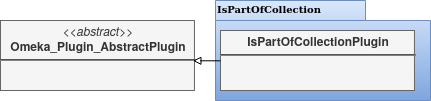
\includegraphics{../_static/images/pck-9.png}
\caption{Diagrama de clases del complemento
AutoDublinCore}\label{da-pck-9}
}
\end{figure}

\begin{figure}
\hypertarget{da-pck-10}{%
\centering
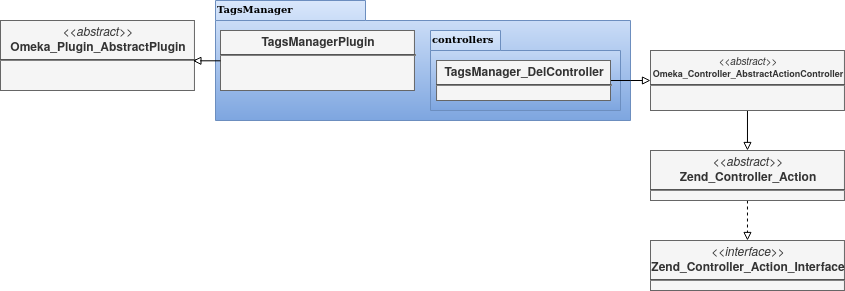
\includegraphics{../_static/images/pck-10.png}
\caption{Diagrama de clases del complemento
TagsManager}\label{da-pck-10}
}
\end{figure}

\hypertarget{diseuxf1o-procedimental}{%
\section{Diseño procedimental}\label{diseuxf1o-procedimental}}

En este apartado se muestra cómo interactúan los principales componentes
de la aplicación ante un determinado evento.

En el diagrama de secuencia que se expone a continuación, se describe el
funcionamiento interno de la aplicación ante una situación general donde
el usuario accede a la aplicación para llevar a cabo una determinada
acción.

\begin{figure}
\hypertarget{dp-seq}{%
\centering
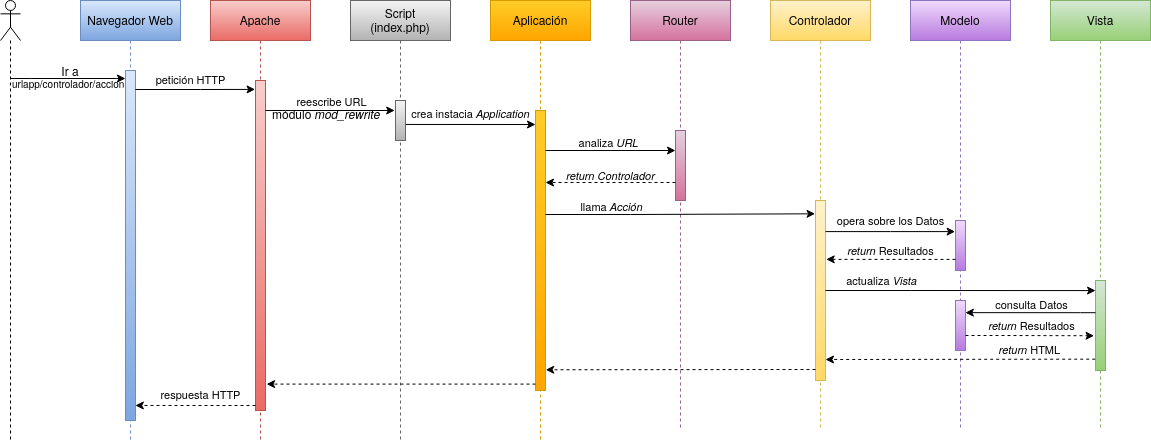
\includegraphics{../_static/images/dp-seq.png}
\caption{Diagrama de secuencia para un caso general.}\label{dp-seq}
}
\end{figure}

En este caso se presupone que tanto el \emph{controlador} como la
\emph{acción} indicada por el usuario son válidas. En caso contrario, se
enviarían las excepciones correspondientes.

\hypertarget{diseuxf1o-de-interfaces}{%
\section{Diseño de interfaces}\label{diseuxf1o-de-interfaces}}

Para la creación del complemento \emph{AriadnePlusTracking} se llevaron
a cabo una serie de prototipos que sirvieron de ayuda visual en las
fases posteriores de desarrollo.

\begin{figure}
\hypertarget{index-prototipe}{%
\centering
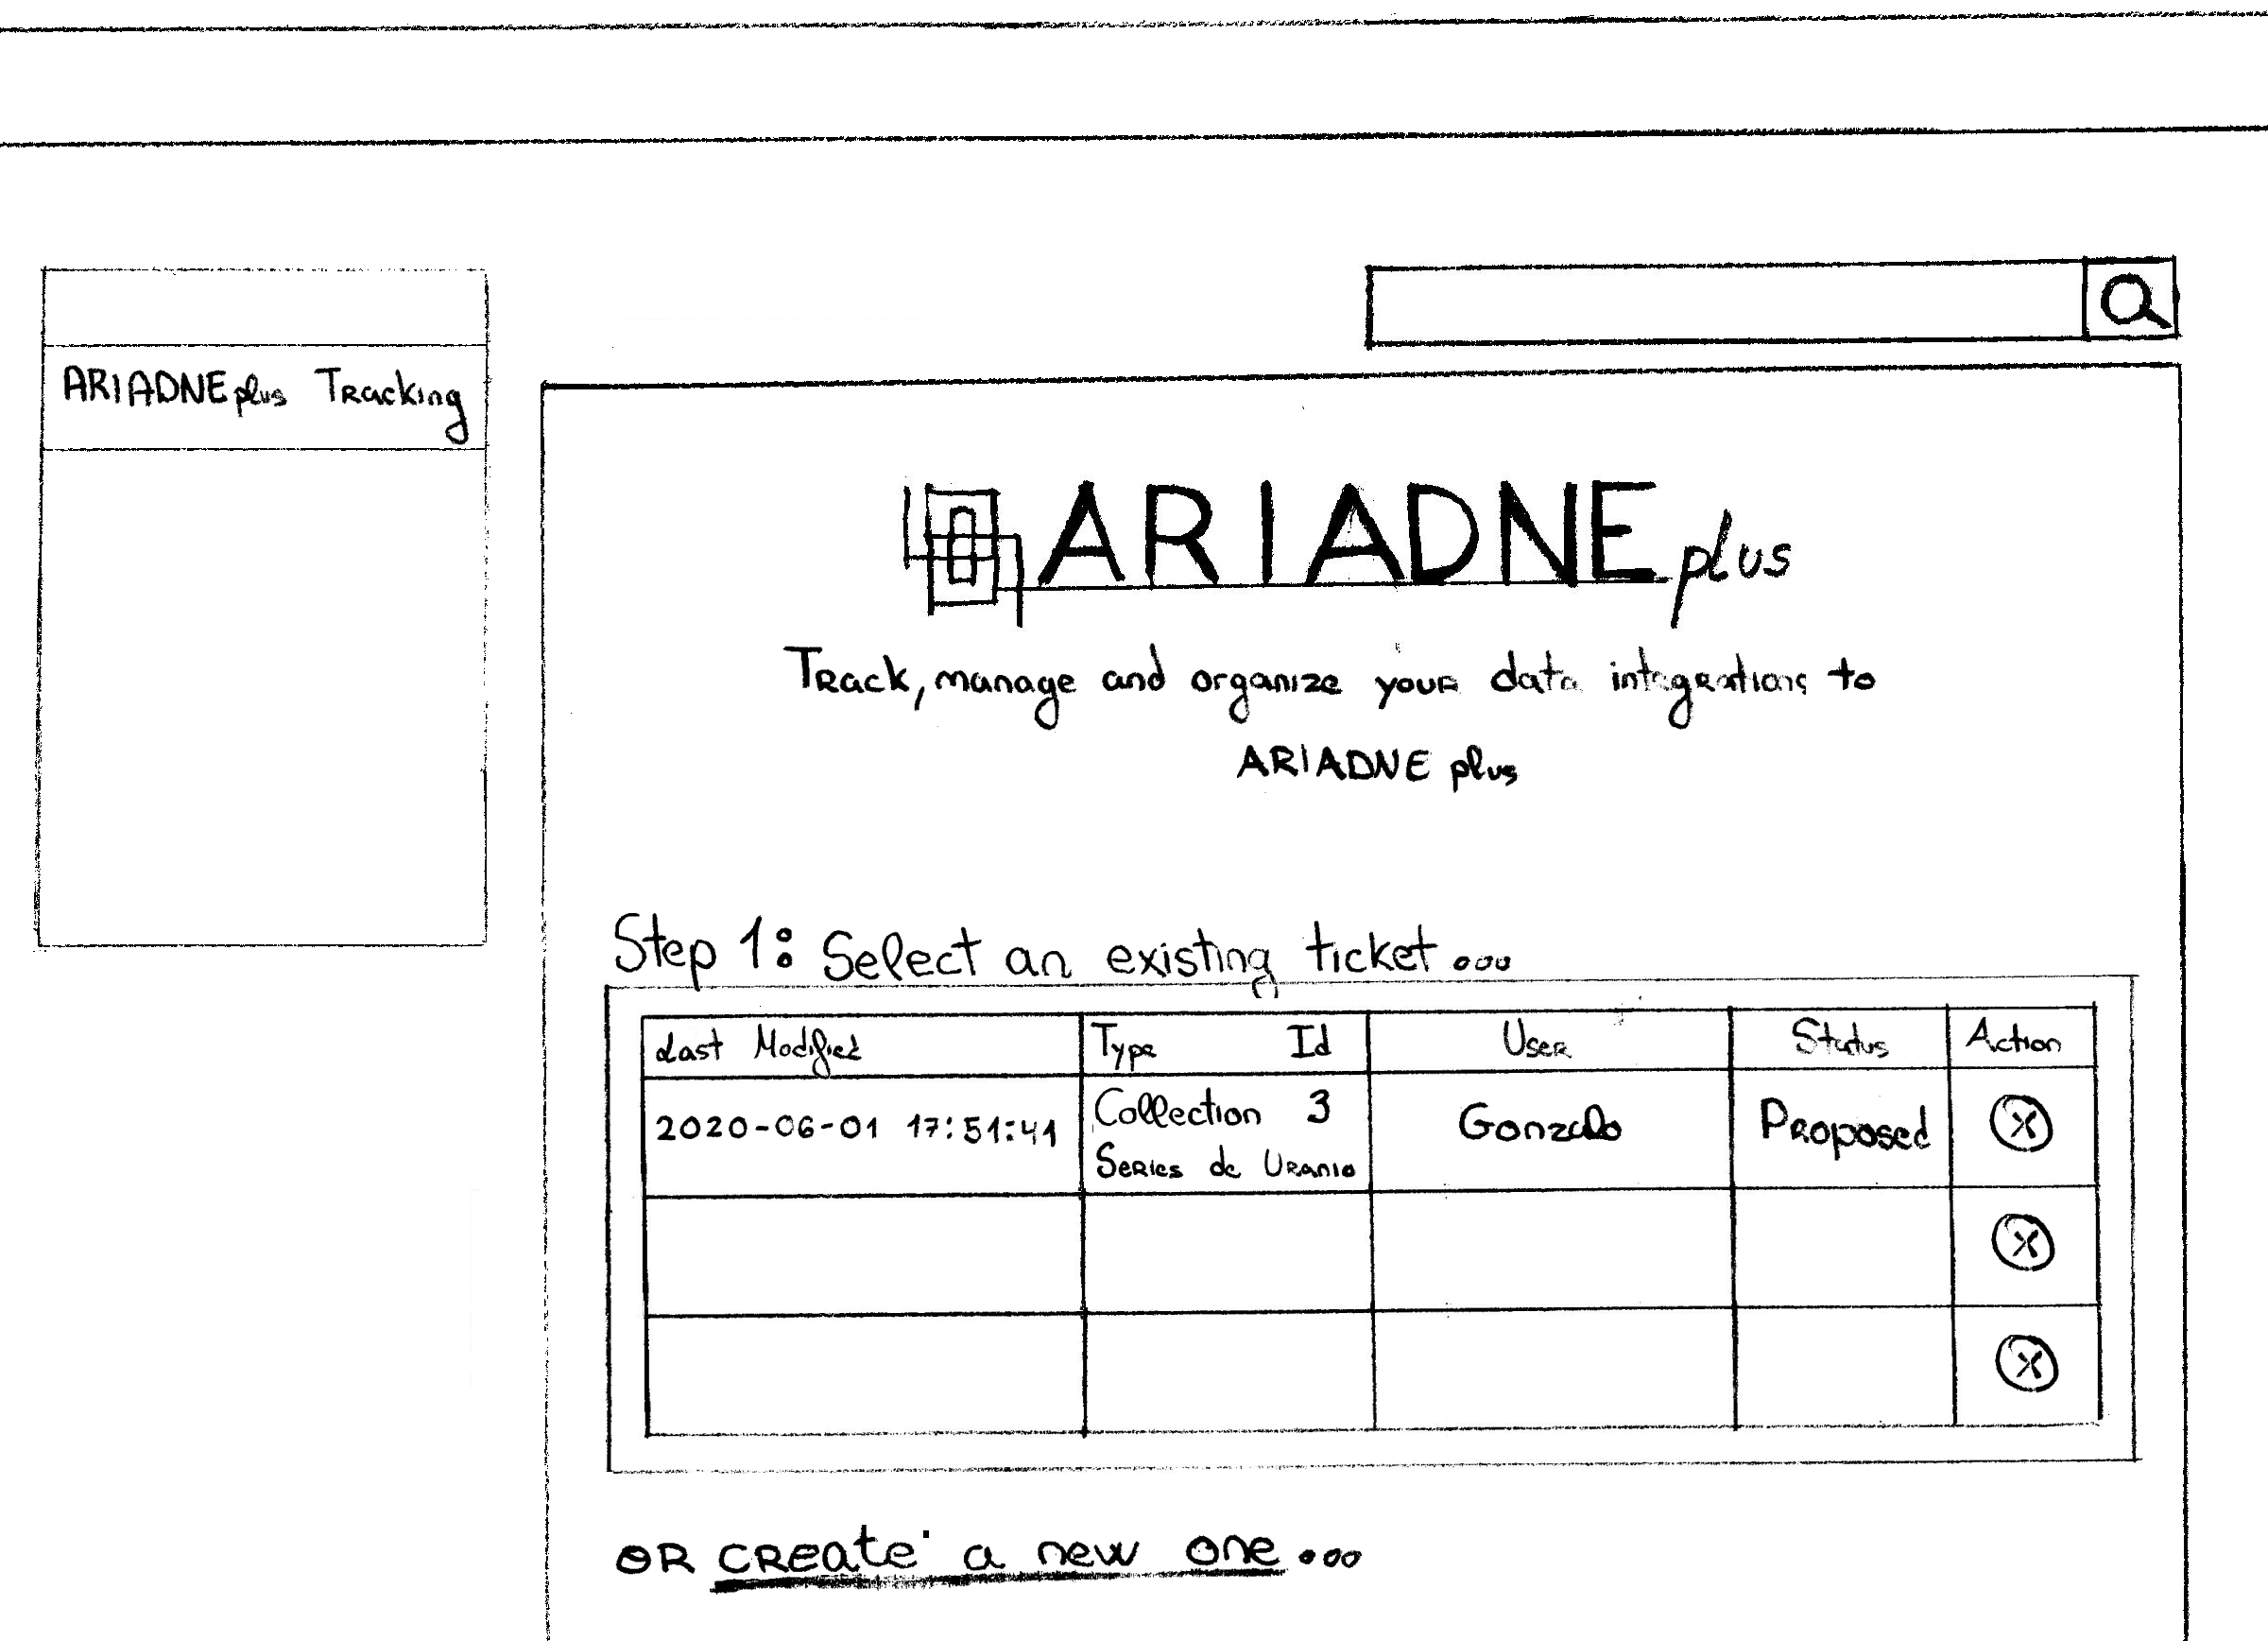
\includegraphics{../_static/images/index-prototipe.png}
\caption{Prototipos: página principal (ARIADNEplus
Tracking)}\label{index-prototipe}
}
\end{figure}

\begin{figure}
\hypertarget{new-prototipe}{%
\centering
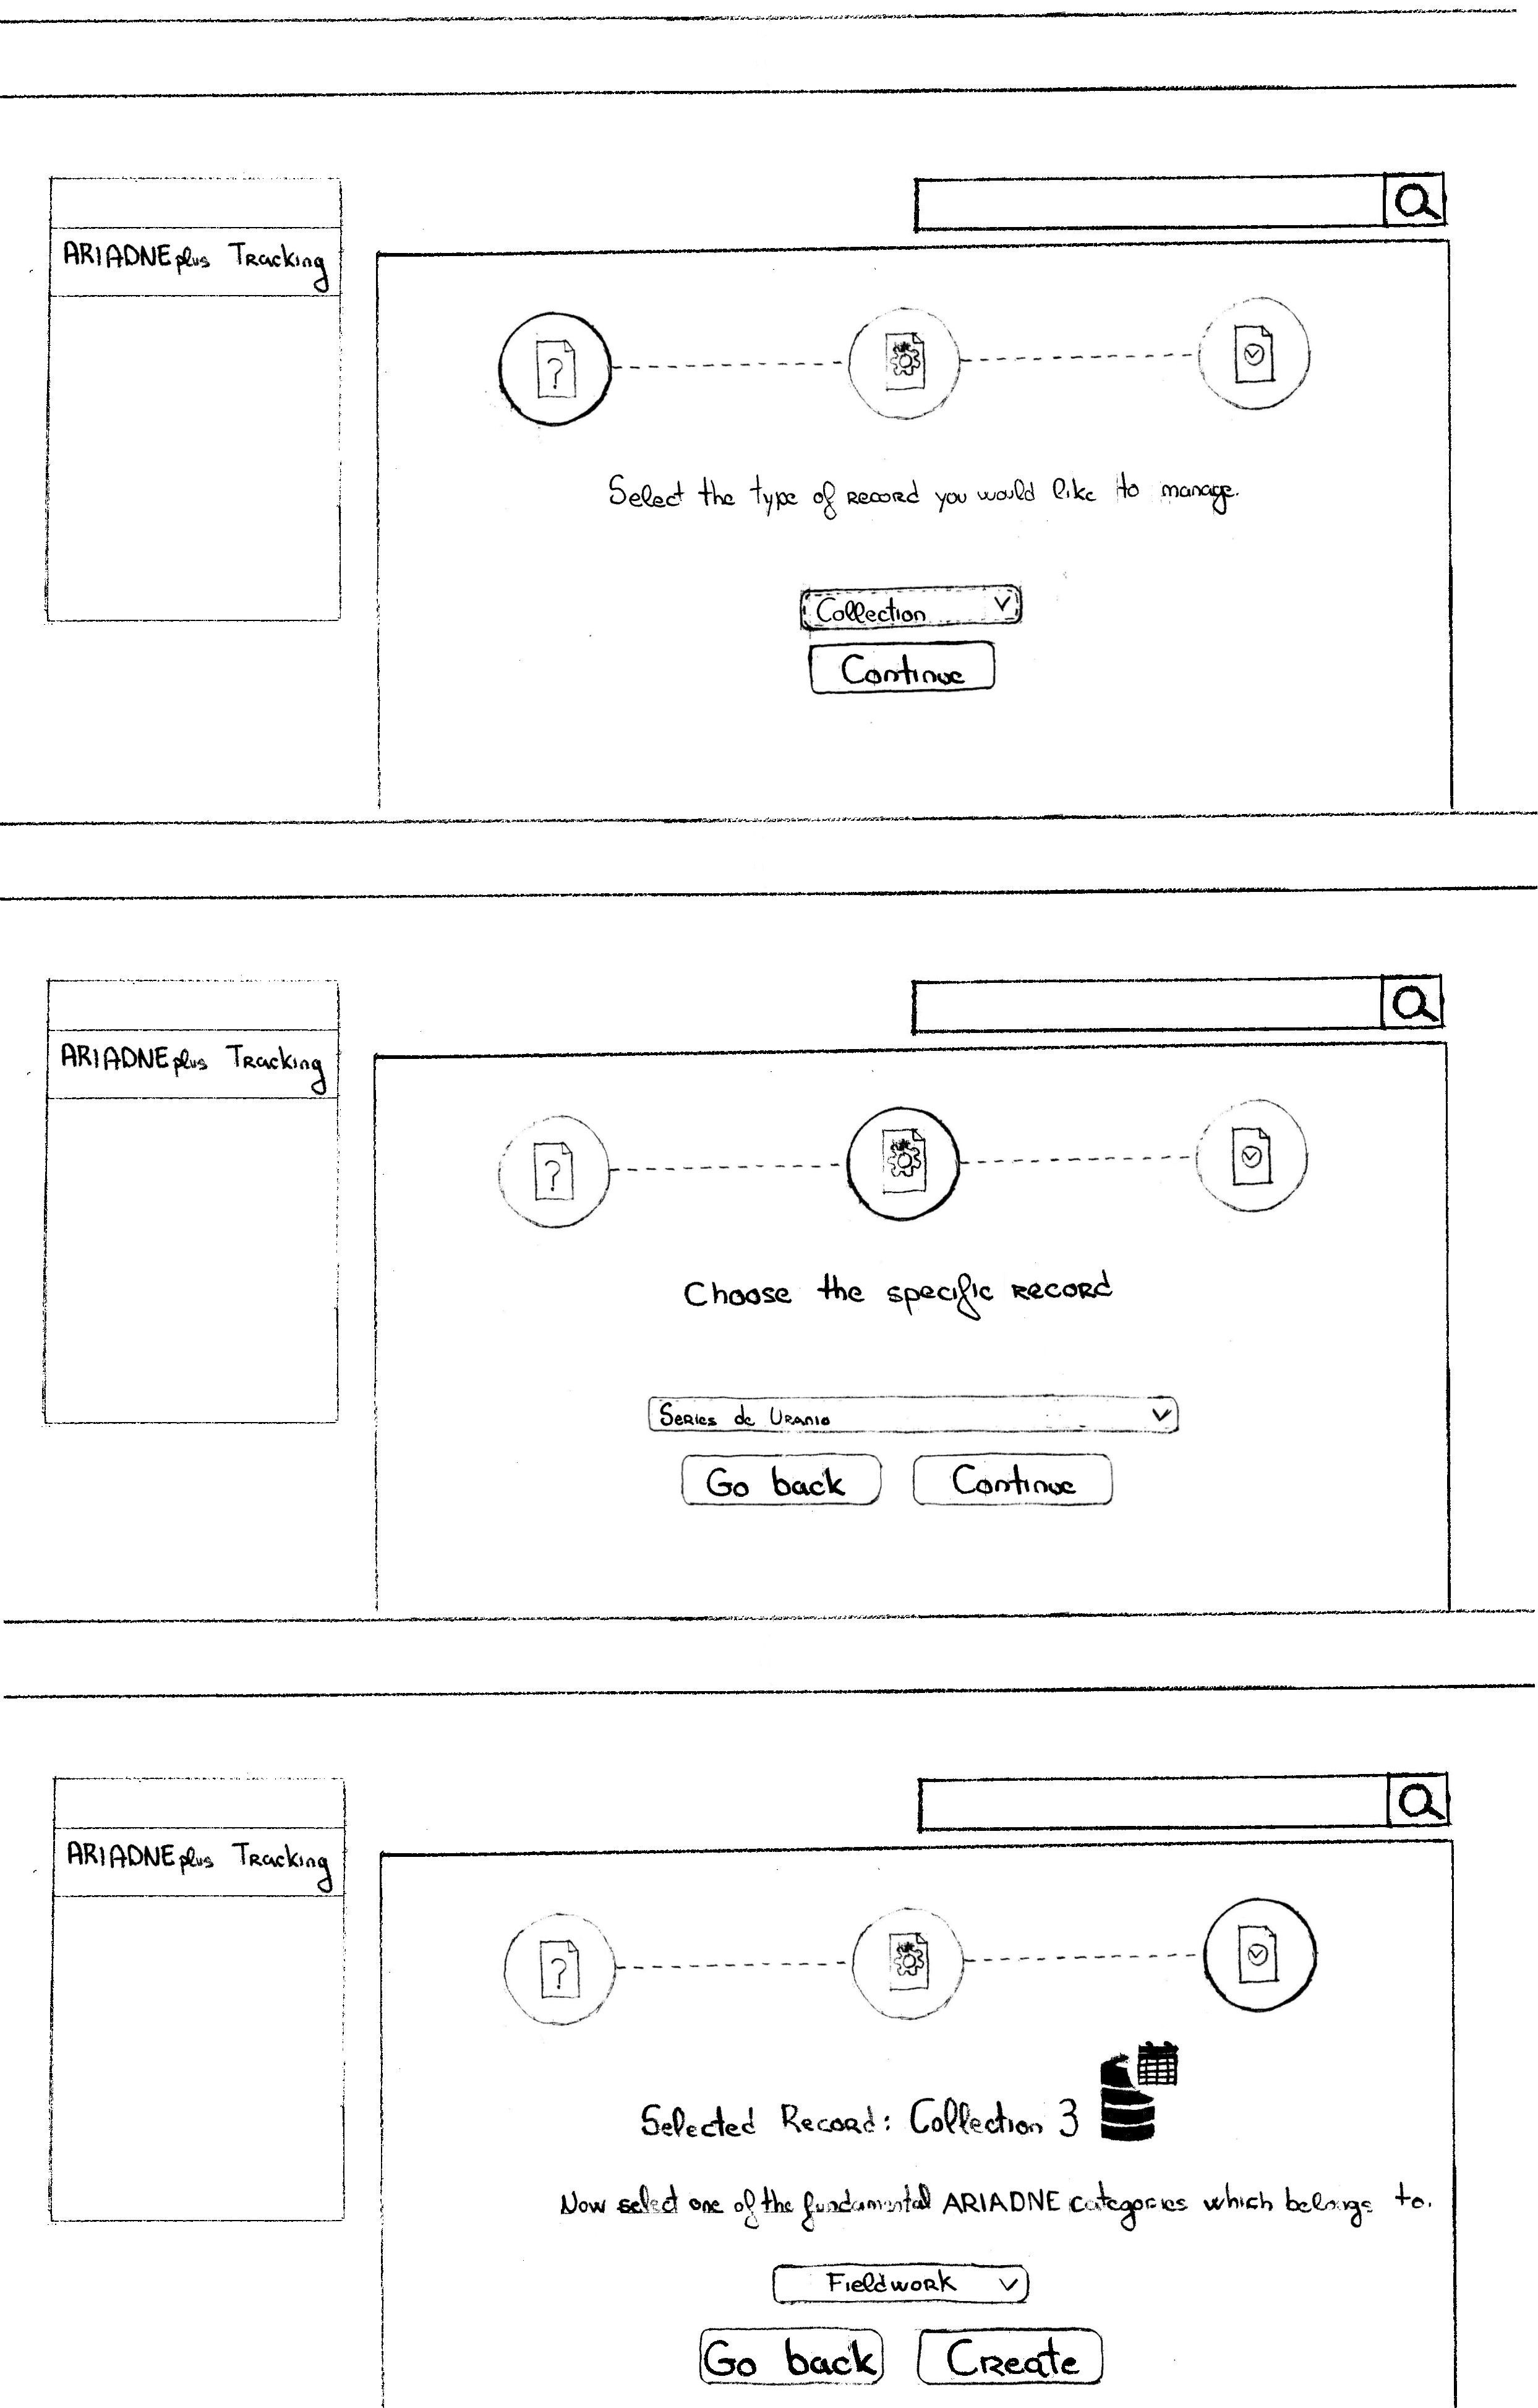
\includegraphics{../_static/images/new-prototipe.png}
\caption{Prototipos: creación de un ticket (ARIADNEplus
Tracking)}\label{new-prototipe}
}
\end{figure}

\begin{figure}
\hypertarget{phase-1-2-prototipe}{%
\centering
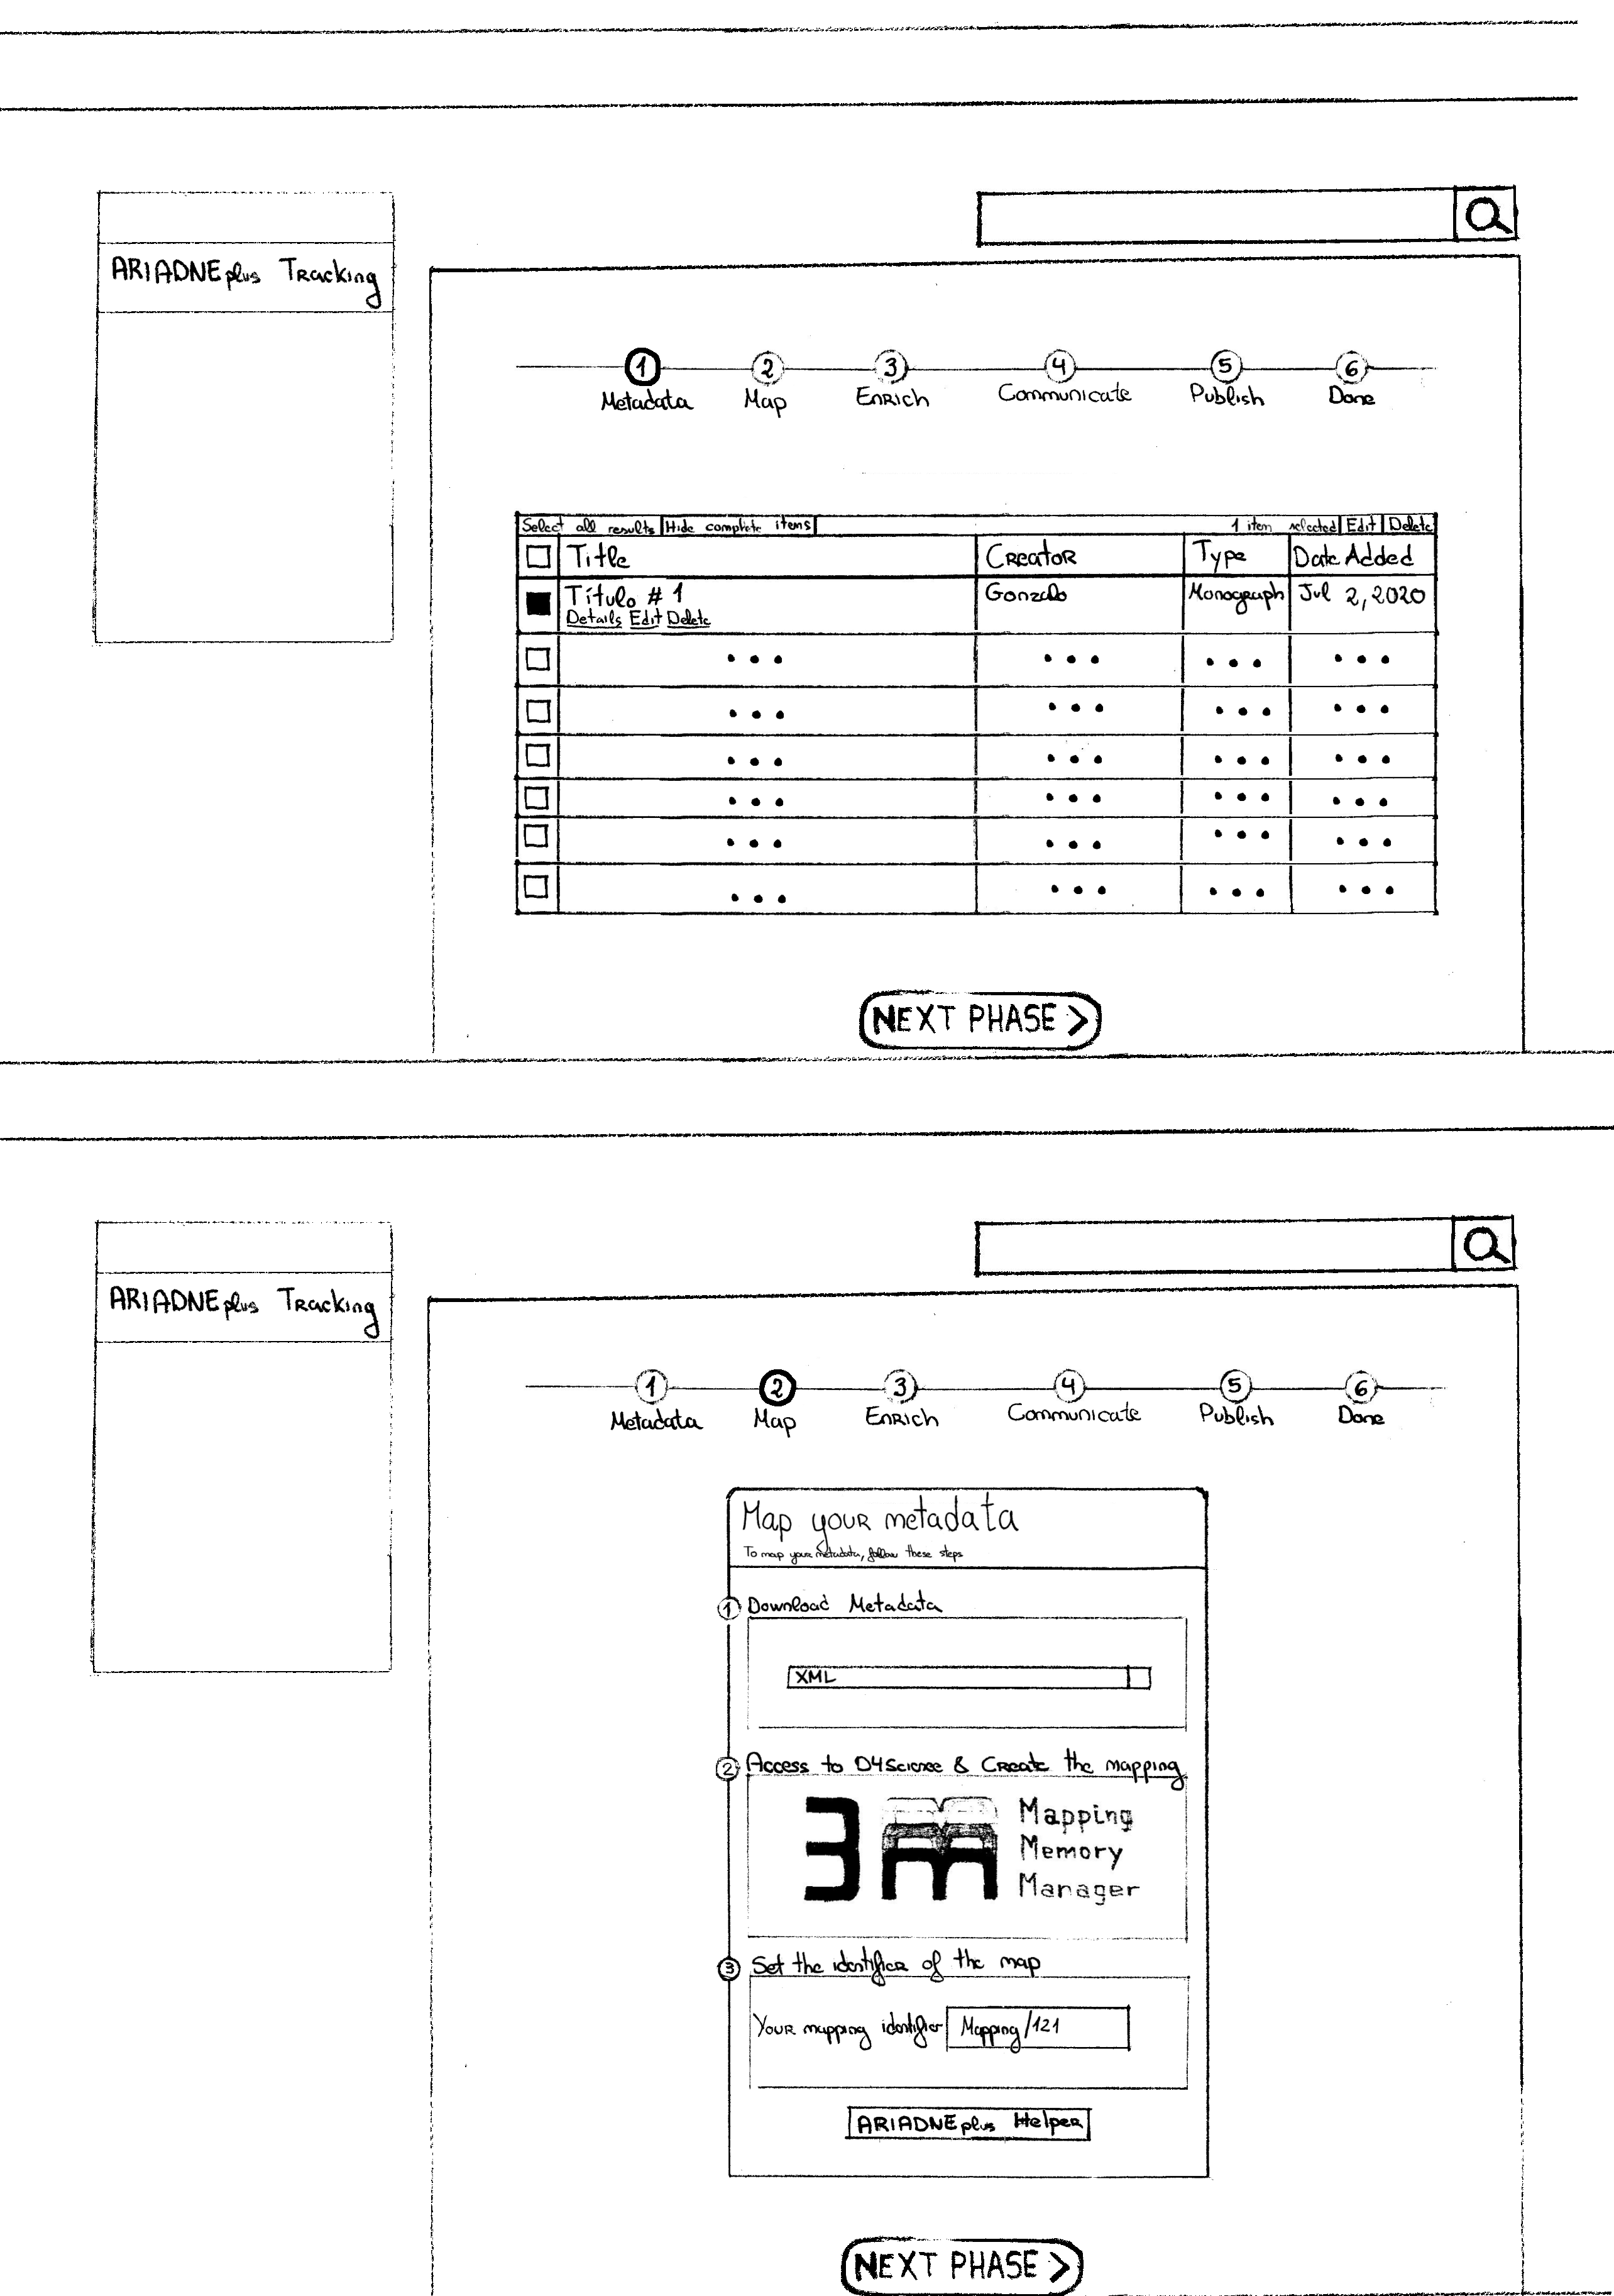
\includegraphics{../_static/images/phase-1-2-prototipe.png}
\caption{Prototipos: primera y segunda fase de un ticket (ARIADNEplus
Tracking)}\label{phase-1-2-prototipe}
}
\end{figure}

\begin{figure}
\hypertarget{phase-3-4-prototipe}{%
\centering
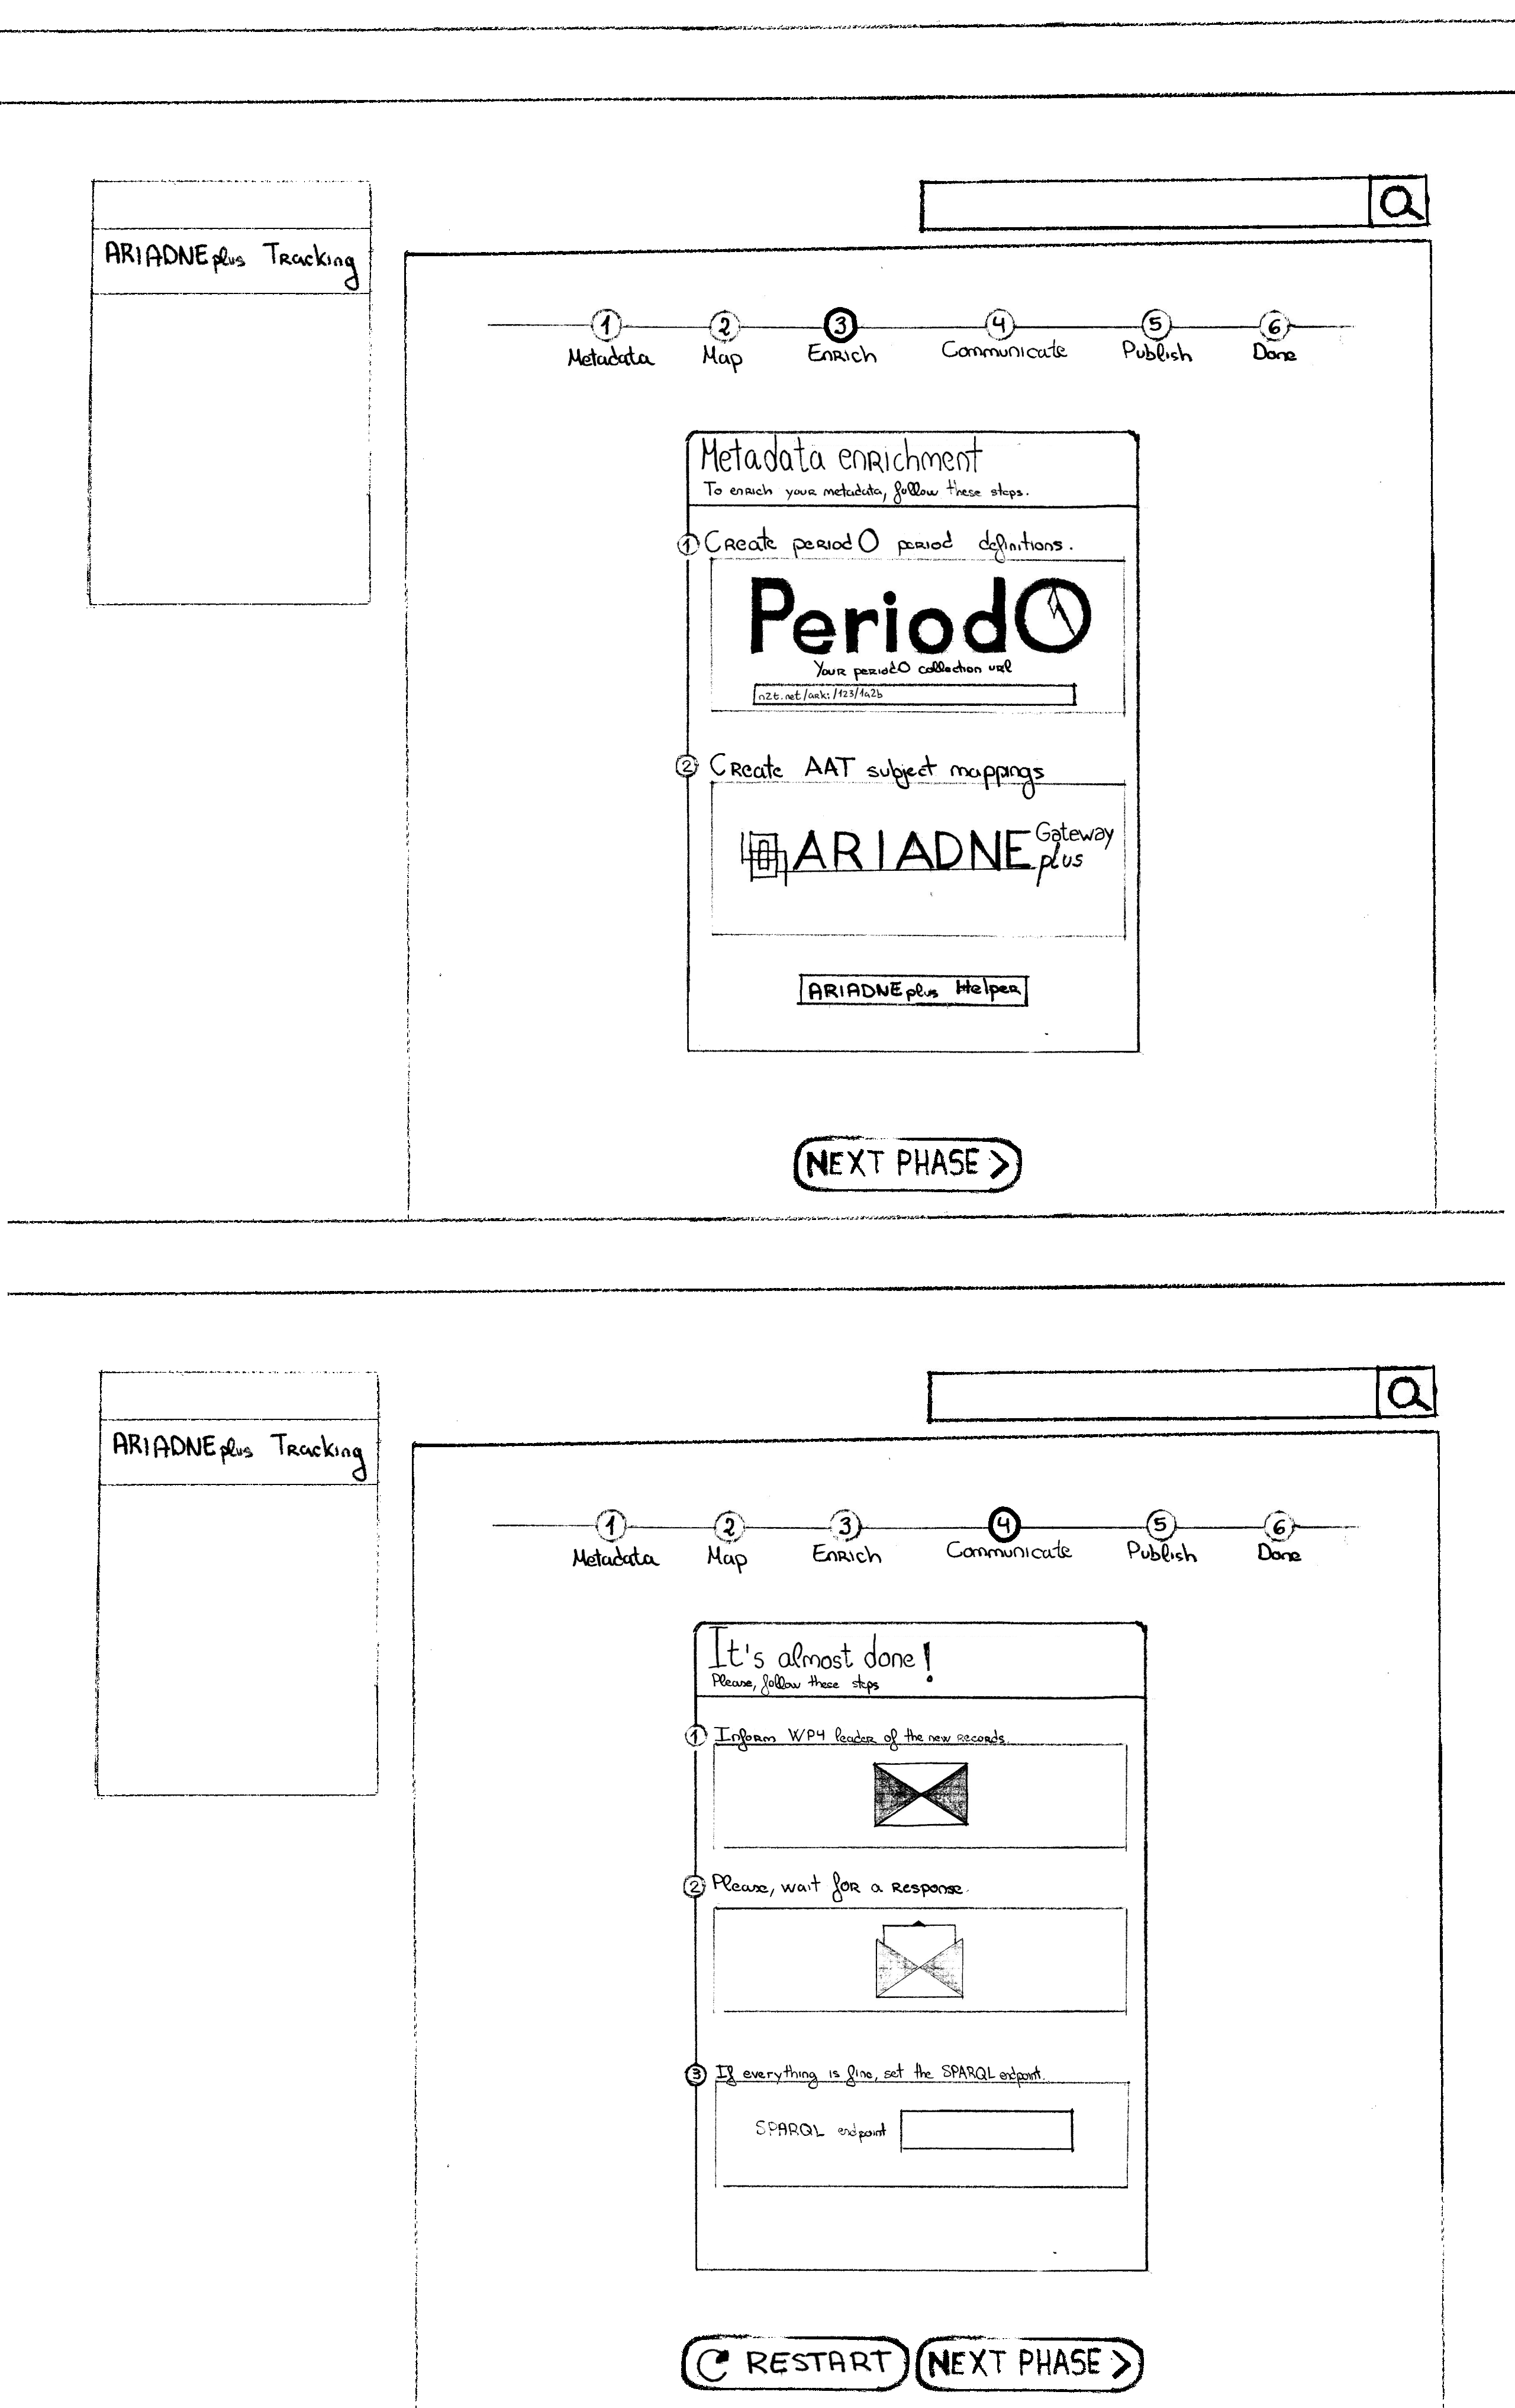
\includegraphics{../_static/images/phase-3-4-prototipe.png}
\caption{Prototipos: tercera y cuarta fase de un ticket (ARIADNEplus
Tracking)}\label{phase-3-4-prototipe}
}
\end{figure}

\begin{figure}
\hypertarget{phase-5-6-prototipe}{%
\centering
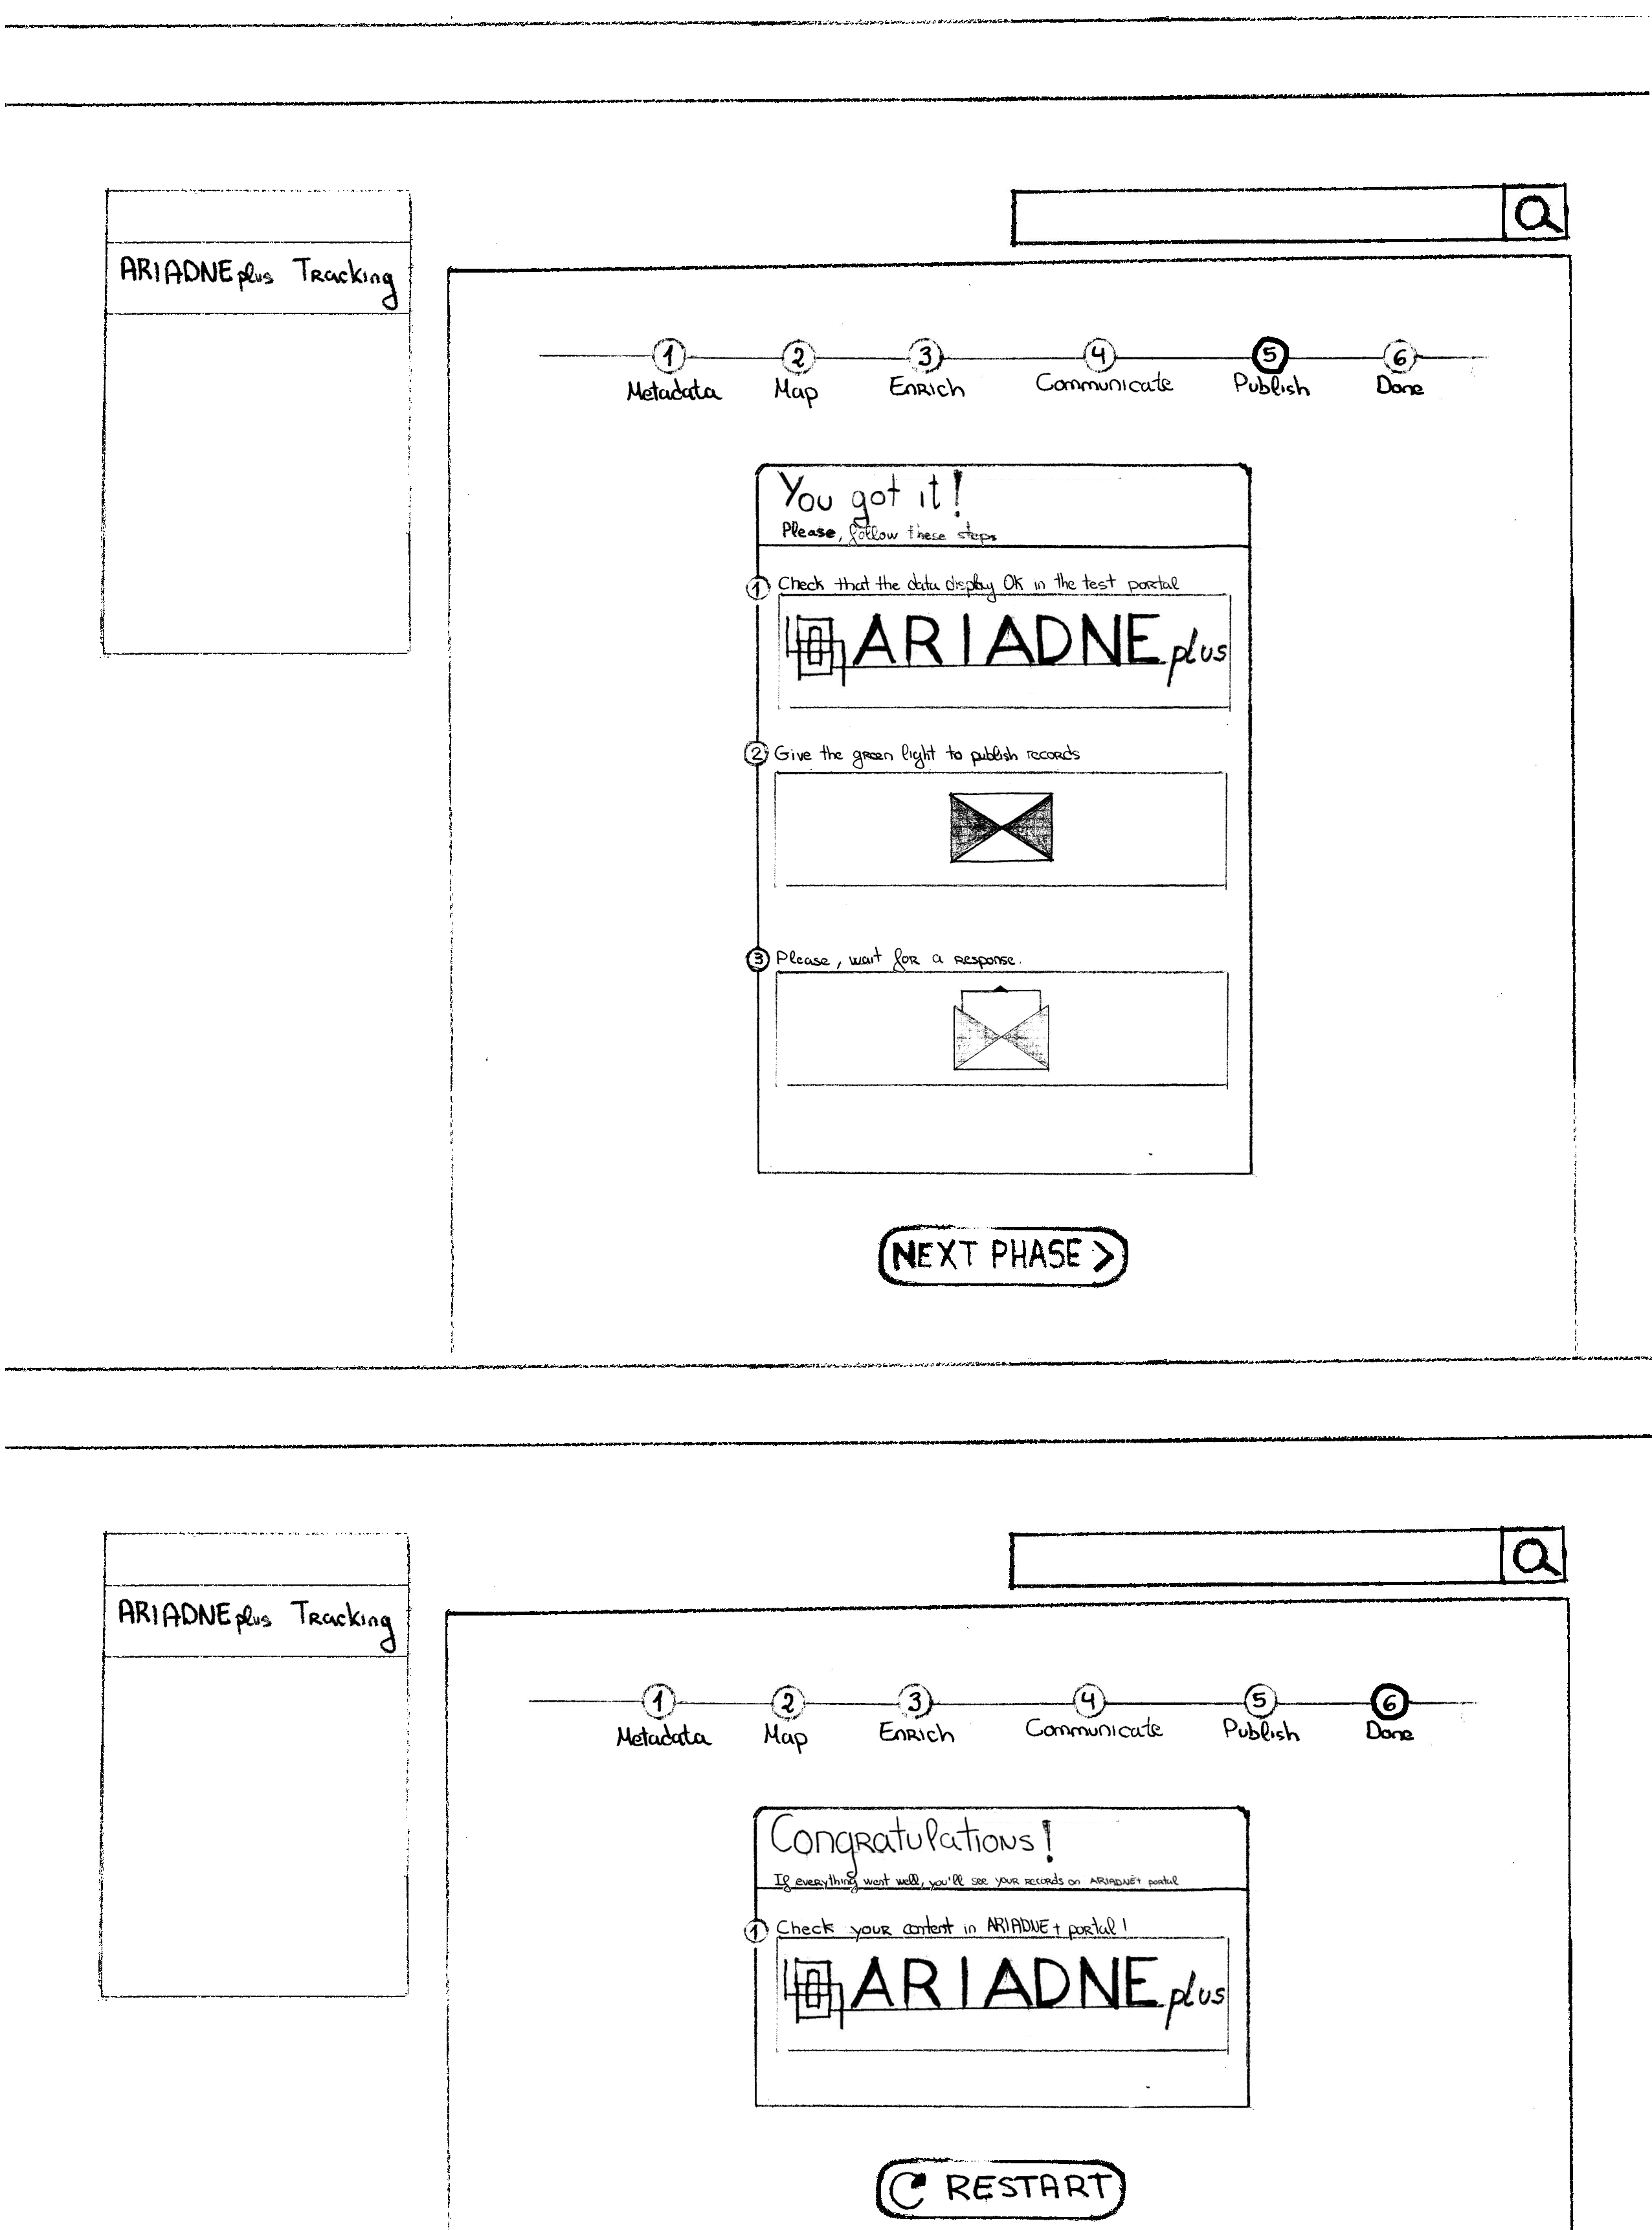
\includegraphics{../_static/images/phase-5-6-prototipe.png}
\caption{Prototipos: quinta y sexta fase de un ticket (ARIADNEplus
Tracking)}\label{phase-5-6-prototipe}
}
\end{figure}

\end{document}
